\documentclass[12pt, a4paper]{article}

% Document setup
\usepackage[english]{babel}
\usepackage[margin=2.5cm]{geometry}

% Graphics
\usepackage{float}
\usepackage{graphicx}
\graphicspath{ {../figures/} }

% Tables
\usepackage{booktabs}
\usepackage{tabularx}

% Math
\usepackage{amsmath, amsthm}

% Referencing
\usepackage[nameinlink]{cleveref}


% Hypotheses setup
\theoremstyle{remark}
\newtheorem*{nullhypothesis}{Null Hypothesis ($H_0$)}
\newtheorem*{alternativehypothesis}{Alternative Hypothesis ($H_A$)}


\begin{document}

\section{Experiment Design and Setup}

\begin{figure}[H]
	\centering
	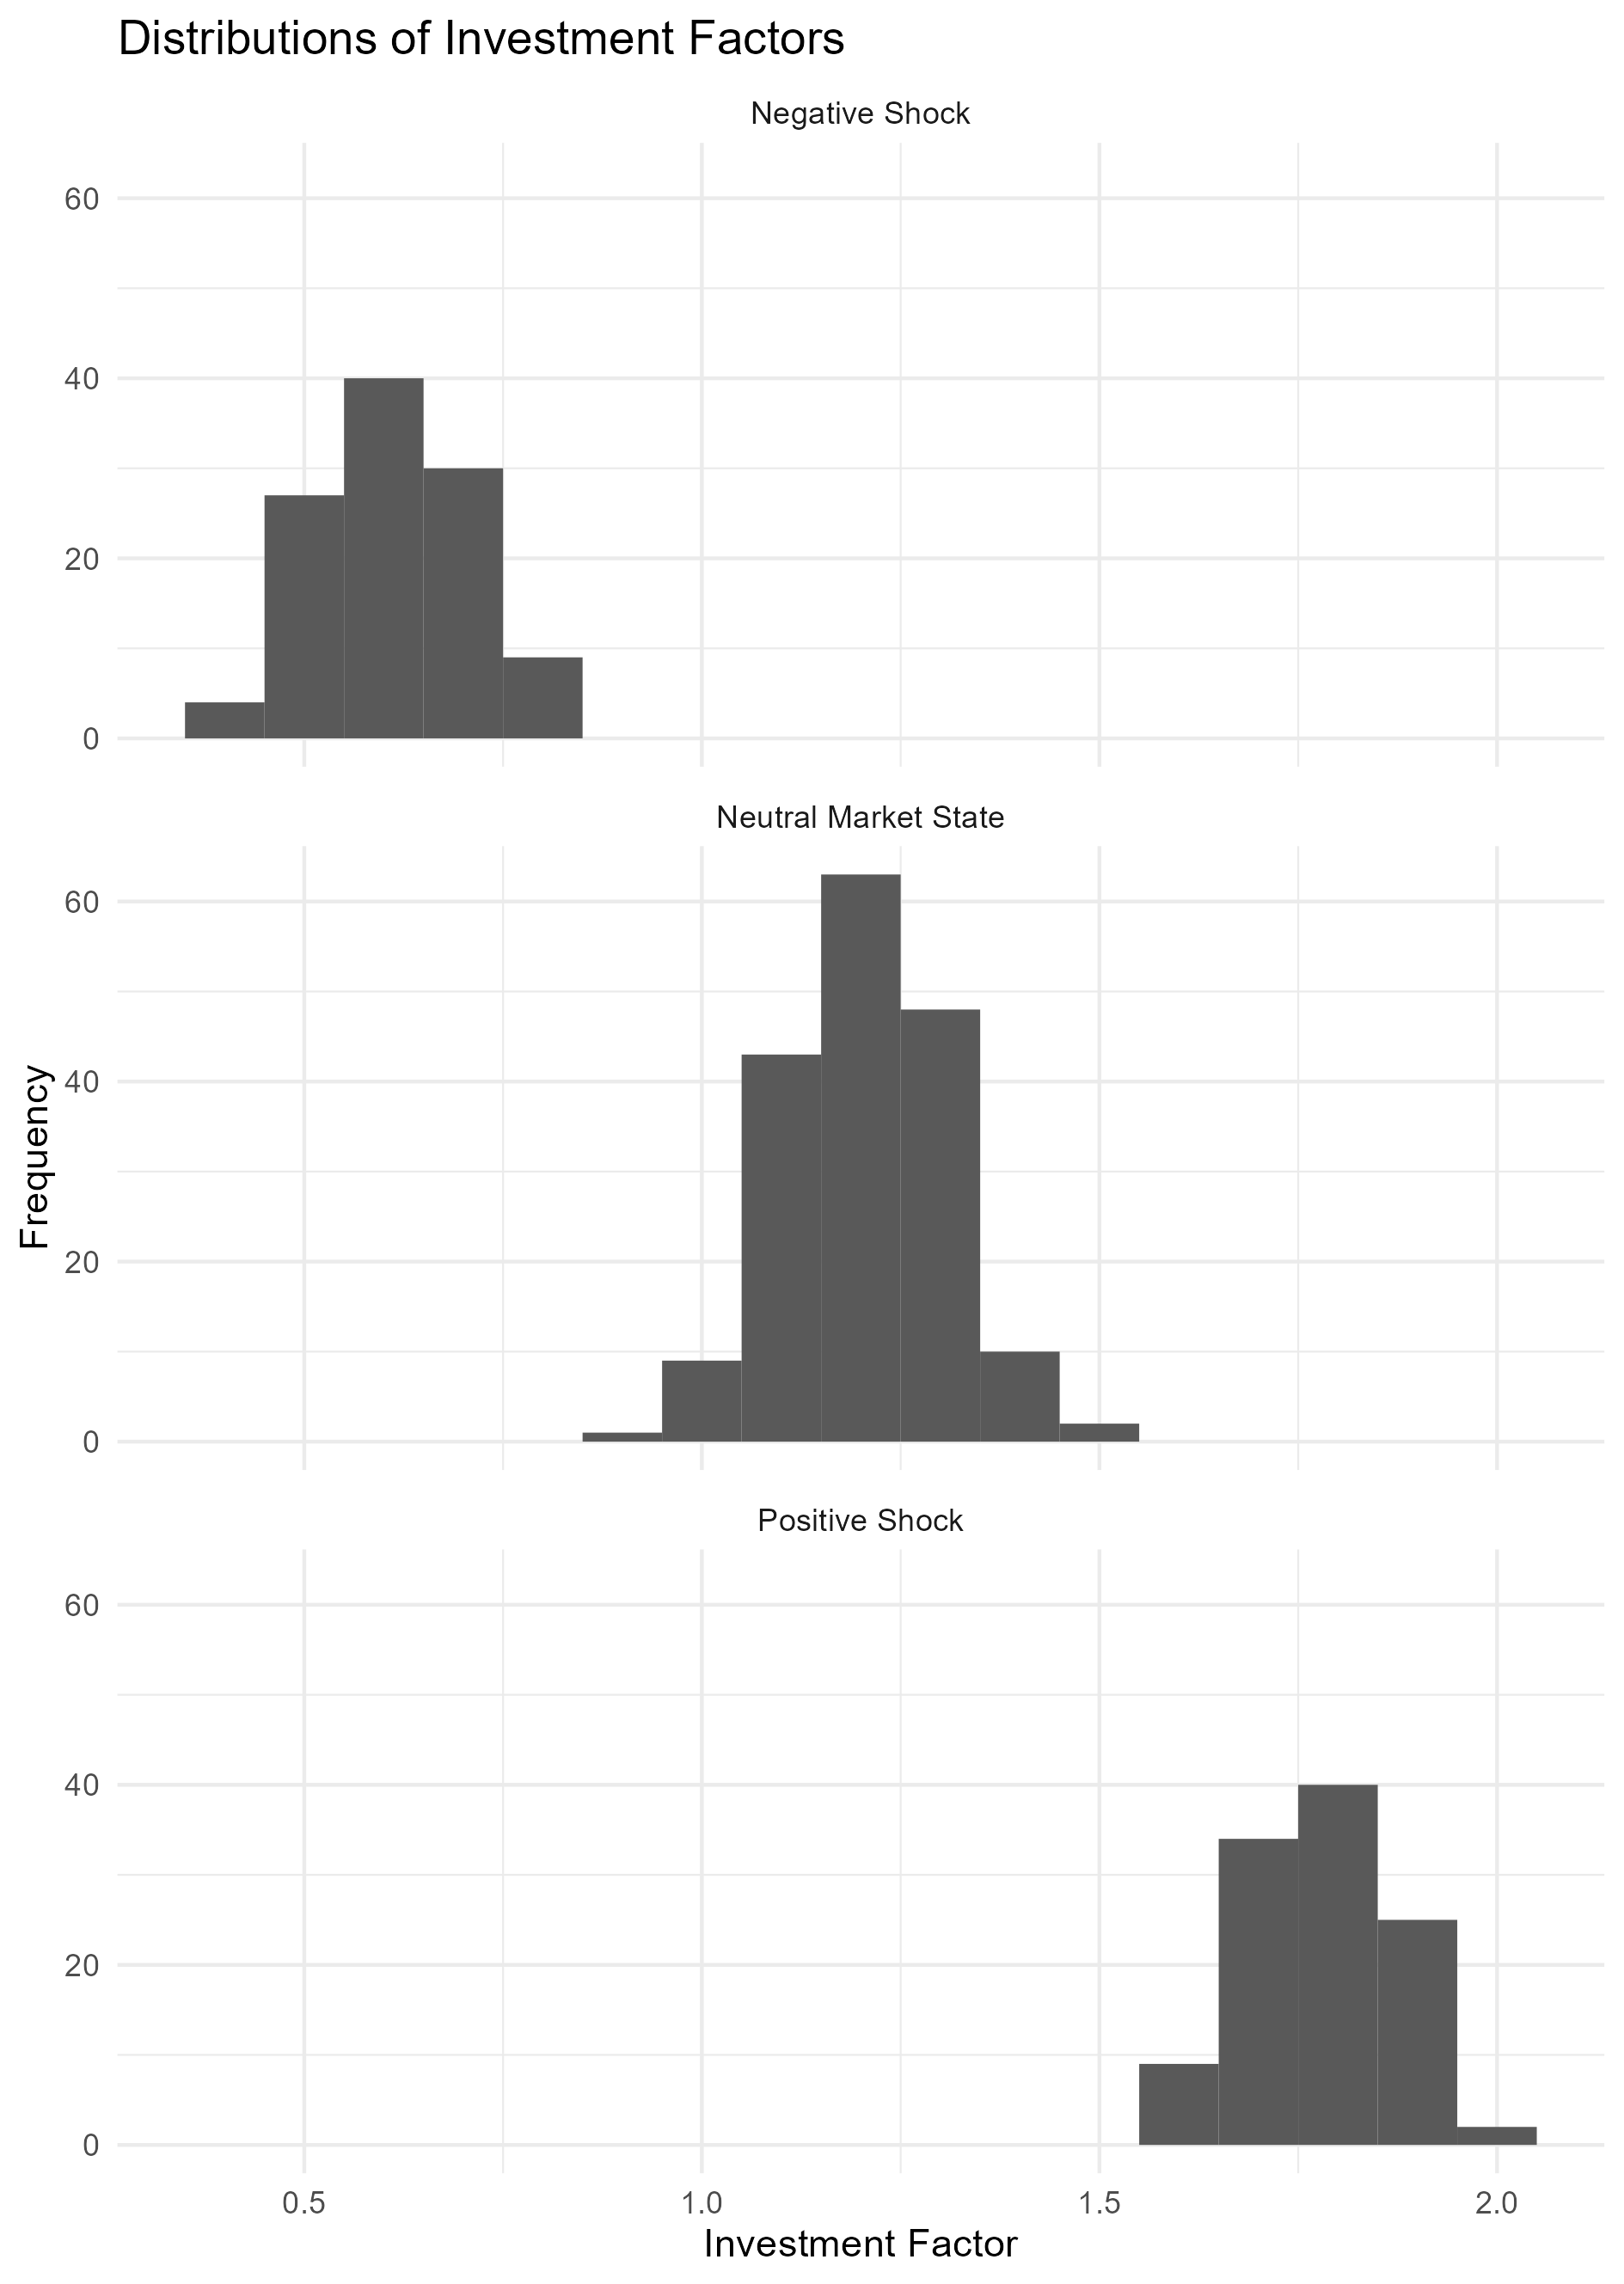
\includegraphics[width=0.7\textwidth]{investment-factors-distributions}
\end{figure}


\section{Aggregate Statistics}

\begin{table}[ht]
\centering
\caption{Investments Summary Statistics (30 Observations)} 
\label{table:InvestmentsSummaryStats}
\begin{tabularx}{\textwidth}{Xrrrr}
  \toprule
Variable & Mean & SD & Min & Max \\ 
  \midrule
Investment Decision Week 4 & 8.700 & 1.968 & 4 & 10 \\ 
  Investment Decision Week 8, Negative Shock Market & 7.533 & 3.889 & 0 & 10 \\ 
  Investment Decision Week 8, Positive Shock Market & 7.190 & 4.174 & 0 & 10 \\ 
  Investment Decision Deviation, Negative Shock Market & -1.467 & 3.583 & -10 & 3 \\ 
  Investment Decision Deviation, Positive Shock Market & -1.210 & 4.066 & -10 & 5 \\ 
   \bottomrule
\end{tabularx}
\end{table}


30 observations in the sample of which half (15) were exposed to a negative and the other half (15) exposed to a positive shock.

At the end of week 4, individuals invested on average 8.7 euros out of their 10 euros. At the end of week 8, individuals who experienced a negative market shock invested on average 7.53 euros and individuals who experienced a positive marketed shock invested 7.19 out of their 10 euros.

\begin{figure}[H]
	\centering
	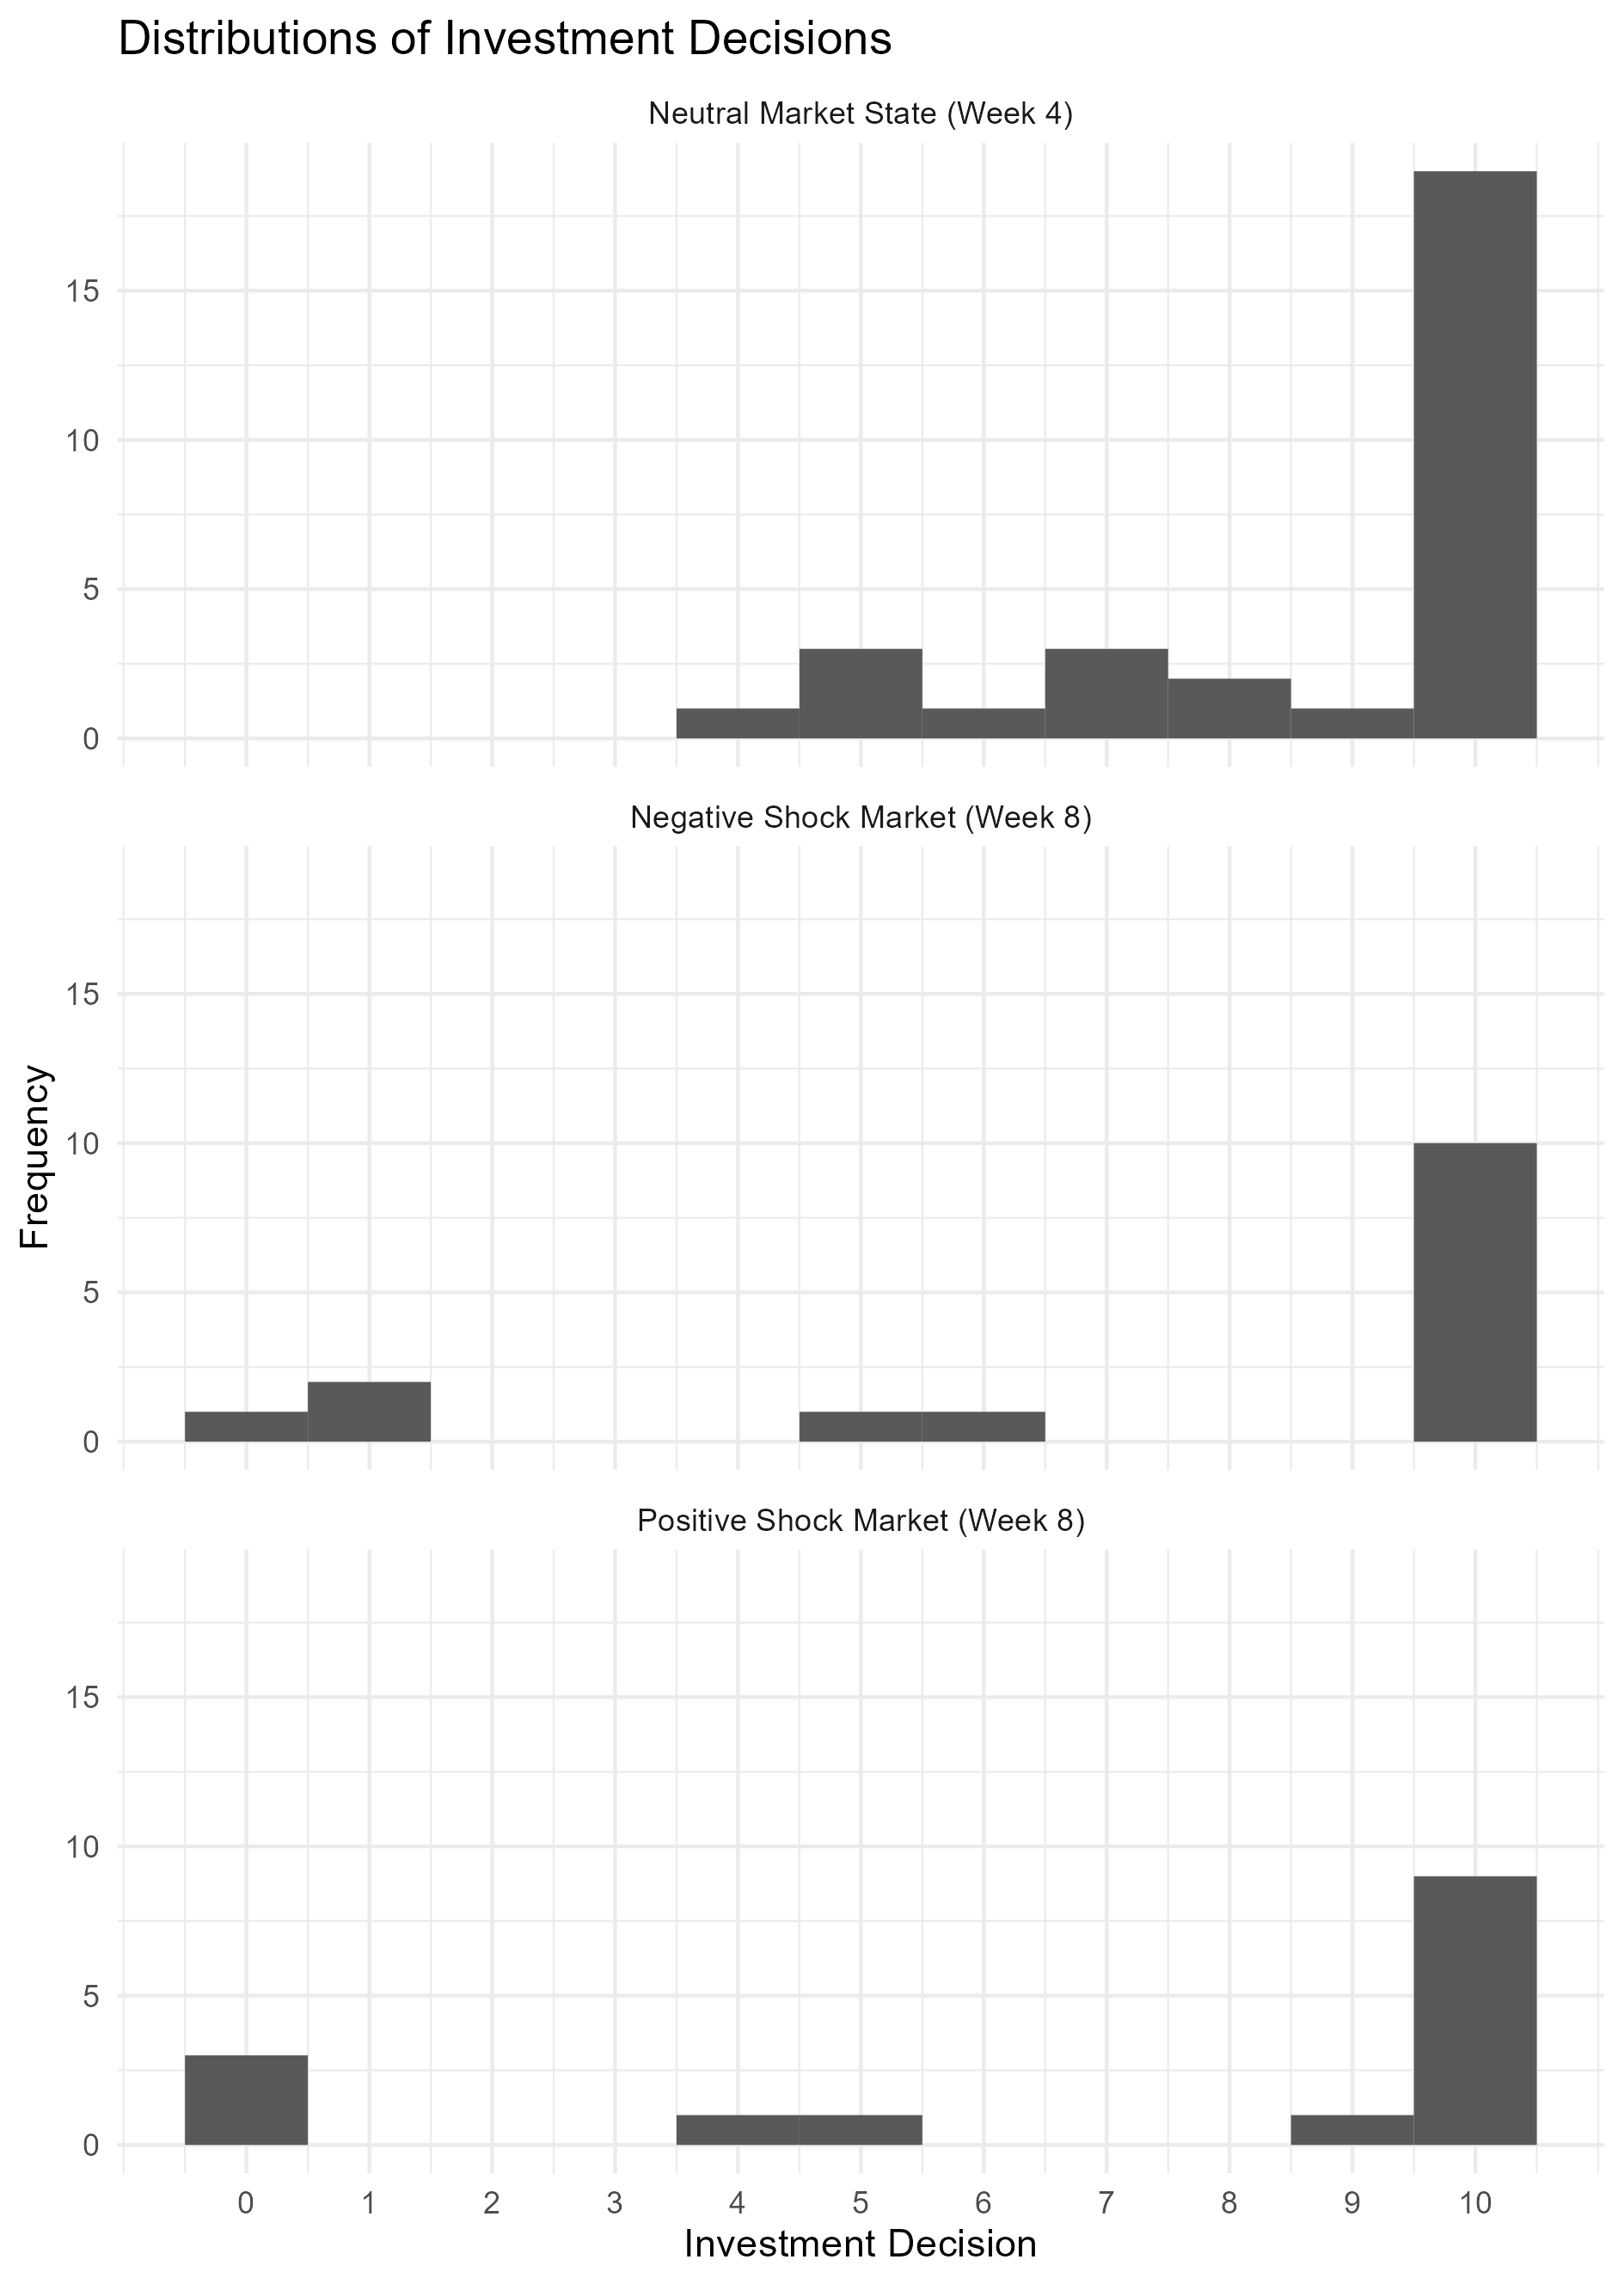
\includegraphics[width=0.7\textwidth]{investment-decisions-distributions}
\end{figure}

\begin{figure}[H]
	\centering
	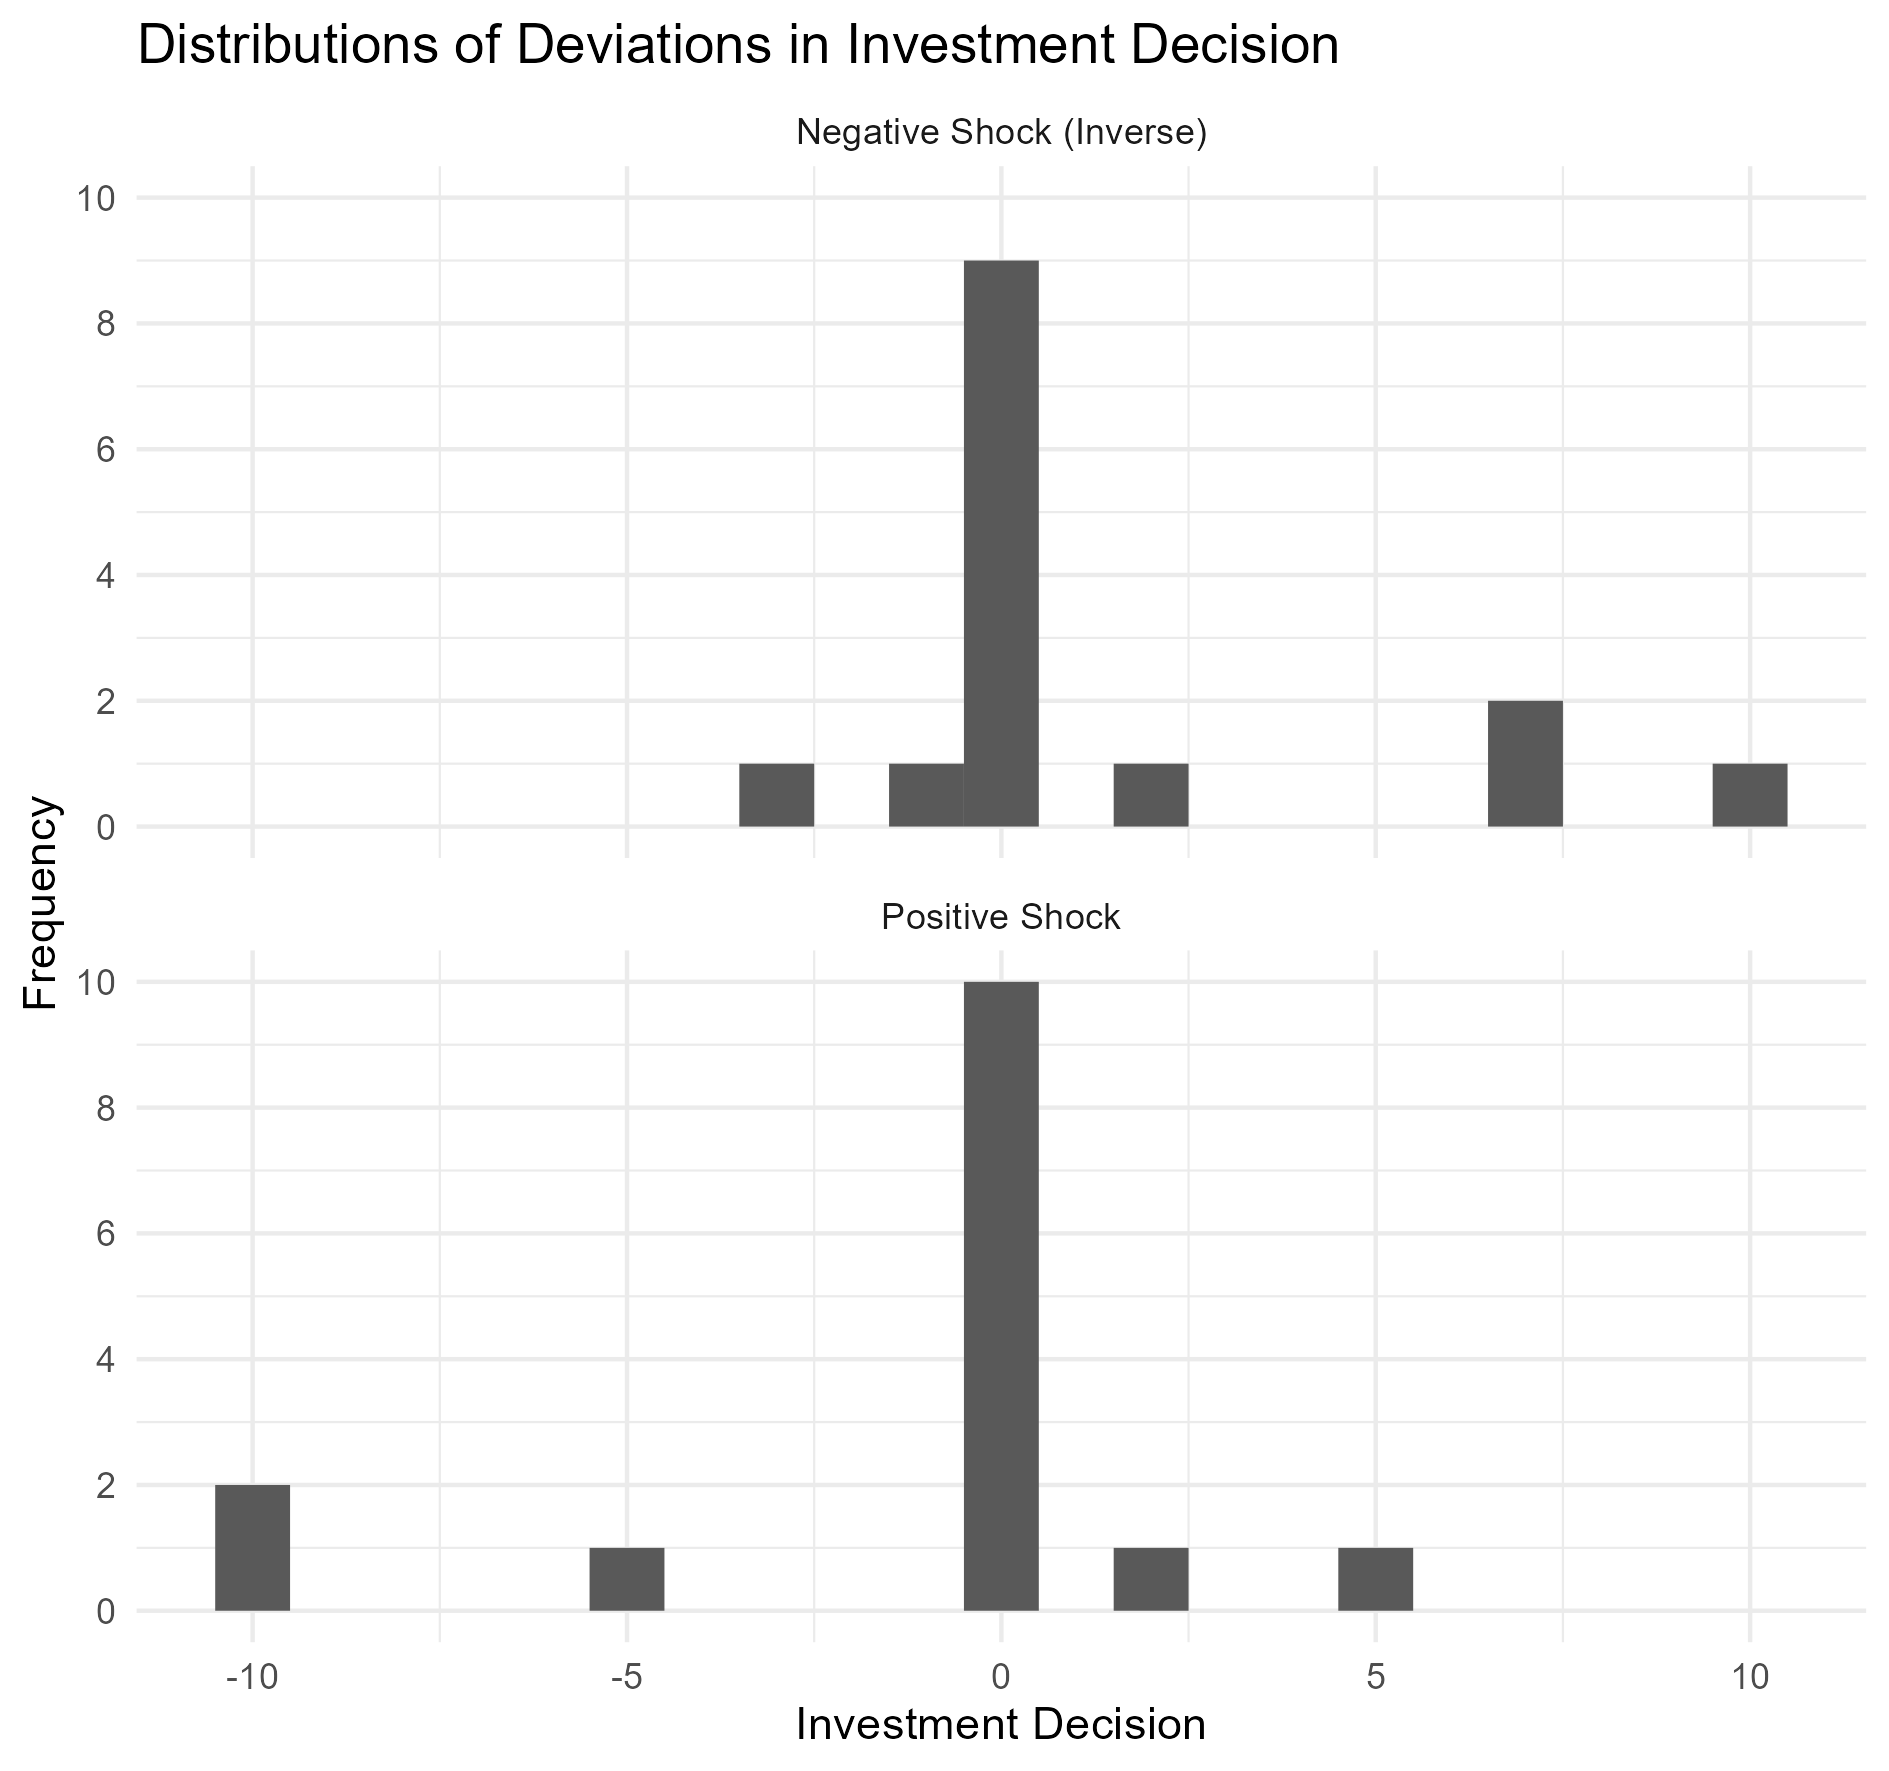
\includegraphics[width=0.7\textwidth]{investment-decision-deviations-distributions}
\end{figure}


\section{Data Analysis}

\subsection{Difference in Differences Analyses}

The negative market shock decreases the mean investment decision by 0.26 (-0.26) euros more compared to the positive market shock. And with that, the average amount of money invested decreases more following a negative shock compared to a positive one. Alternatively, the positive market shock decreases the mean investment decision by 0.26 euros less compared to the negative market shock.

The negative market shock increases the standard deviation by 0.72 euros compared to the positive market shock. And with that, the variability in the investment decision distribution increases more following a negative market shock compared to the case of a positive market shock.


\subsection{Mann-Whitney U Test}

\begin{nullhypothesis}
Individuals react symmetrically to positive and negative shocks. Thus, the deviation in the investment decision values in the positive shock market and the inverse deviation in the investment decision values in the negative shock market are equal.
\end{nullhypothesis}

\begin{alternativehypothesis}
Individuals react asymmetrically to positive and negative shocks. Thus, the deviation in the investment decision values in the positive shock market and the inverse deviation in the investment decision values in the negative shock market are not equal.
\end{alternativehypothesis}

We fail to reject the null hypothesis since the $p\text{-value} = 0.2491 > p\text{-critical} = 0.10$. The change in the investment decisions following a positive market shock is not significantly different to the inverse change in the investment decisions following a negative market shock.

\subsubsection{Subgroup Analysis}

Subsample using only observations of individuals who changed their investment decision after the market shocks: We reject the null hypothesis in favor of the alternative hypothesis since $p\text{-value} = 0.0814 < p-critical = 0.10$. The change in the investment decisions following a positive market shock is significantly different to the inverse change in the investment decisions following a negative market shock at the 10 percent level.

Subsample using only observations of individuals with at least some trading experience: We fail to reject the null hypothesis since $p\text{-value} = 0.4368 > p\text{-critical} = 0.10$. The change in the investment decisions following a positive market shock is not significantly different to the inverse change in the investment decisions following a negative market shock.

\end{document}